\documentclass[11pt]{article}
\usepackage[margin=1in]{geometry}
\usepackage{graphicx}
\usepackage{subcaption}
\usepackage{booktabs}
\usepackage{float}
\usepackage{hyperref}
\usepackage{longtable}

\title{Evaluation of a Reliability-Based Maintenance Interval Optimizer}
\author{Codex Repository Evaluation}
\date{April 17, 2026}

\begin{document}
\maketitle

\begin{abstract}
This document evaluates the maintenance optimizer implemented in this repository. Synthetic failure datasets were generated to represent low-risk, wear-out, and fragile components. The command-line interface was then exercised across multiple configurations using exponential, Weibull, and combined reliability modeling. The results show that the tool consistently produces reusable metrics, recommendation tables, JSON summaries, and reliability figures. The experiments also show that model choice materially changes maintenance timing: exponential assumptions produce much earlier intervention times than Weibull fits on the same component set, while high-criticality fragile assets trigger very early inspection and maintenance actions.
\end{abstract}

\section{Introduction}
The objective of this evaluation was straightforward: prove that the CLI works end to end, verify that it generates interpretable outputs, and document how maintenance recommendations shift across different data regimes. The study used the implementation in \texttt{src/reliability\_cli/} and saved all generated inputs and outputs under the repository root in \texttt{results/}.

\section{Synthetic Data Generation}
All datasets were generated with a fixed random seed of 42. Six single-component datasets were created for direct analysis, and one multi-component dataset was created for comparison mode. Each single-component CSV contains \texttt{hours} and \texttt{failures} columns. The comparison CSV contains one row per component with explicit Weibull parameters and criticality labels.

\begin{table}[H]
\centering
\caption{Generated single-component datasets}
\begin{tabular}{lrrl}
\toprule
Component & Operating Time & Failures & Intended Behavior \\
\midrule
stable\_motor & 14267 & 8 & Low hazard, slow degradation \\
wearing\_pump & 12696 & 21 & Wear-out dominated \\
fragile\_sensor & 7005 & 22 & Early-life failures / fragile \\
heavy\_valve & 23880 & 20 & Long-lived but non-trivial hazard \\
aging\_bearing & 15021 & 46 & Fast wear-out \\
balanced\_fan & 15780 & 21 & Moderate degradation \\
\bottomrule
\end{tabular}
\end{table}

\section{CLI Evaluation Design}
Nine CLI evaluations were executed:

\begin{enumerate}
\item Six \texttt{analyze} runs, one per dataset
\item Three \texttt{compare} runs on the shared component table
\end{enumerate}

The commands were:

\begin{verbatim}
python -m reliability_cli analyze --input results/datasets/stable_motor.csv \
  --time-col hours --failure-col failures --model both --theta 6200 \
  --beta 1.2 --criticality low --tmax 16000 \
  --out results/evals/stable_motor_both

python -m reliability_cli analyze --input results/datasets/wearing_pump.csv \
  --time-col hours --failure-col failures --model weibull --theta 4200 \
  --beta 2.7 --criticality medium --tmax 14000 \
  --out results/evals/wearing_pump_weibull

python -m reliability_cli analyze --input results/datasets/fragile_sensor.csv \
  --time-col hours --failure-col failures --model both --theta 3000 \
  --beta 0.85 --criticality high --tmax 9000 \
  --out results/evals/fragile_sensor_both

python -m reliability_cli analyze --input results/datasets/heavy_valve.csv \
  --time-col hours --failure-col failures --model exponential \
  --criticality medium --tmax 26000 \
  --out results/evals/heavy_valve_exponential

python -m reliability_cli analyze --input results/datasets/aging_bearing.csv \
  --time-col hours --failure-col failures --model weibull --theta 3600 \
  --beta 3.1 --criticality high --tmax 16000 \
  --out results/evals/aging_bearing_weibull

python -m reliability_cli analyze --input results/datasets/balanced_fan.csv \
  --time-col hours --failure-col failures --model both --theta 5600 \
  --beta 1.6 --criticality low --tmax 17000 \
  --out results/evals/balanced_fan_both

python -m reliability_cli compare --input results/datasets/compare_components.csv \
  --name-col component --time-col operating_time --failure-col failures \
  --theta-col theta --beta-col beta --criticality-col criticality \
  --model weibull --tmax 12000 --out results/evals/compare_weibull

python -m reliability_cli compare --input results/datasets/compare_components.csv \
  --name-col component --time-col operating_time --failure-col failures \
  --theta-col theta --beta-col beta --criticality-col criticality \
  --model both --tmax 12000 --out results/evals/compare_both

python -m reliability_cli compare --input results/datasets/compare_components.csv \
  --name-col component --time-col operating_time --failure-col failures \
  --theta-col theta --beta-col beta --criticality-col criticality \
  --model exponential --tmax 12000 --out results/evals/compare_exponential
\end{verbatim}

\section{Single-Component Results}
Table~\ref{tab:single_results} summarizes the single-component runs. The recommendation times are taken directly from each run's \texttt{summary.json}. Two patterns stand out immediately. First, \texttt{fragile\_sensor} is flagged almost immediately because it combines high failure intensity with high criticality thresholds. Second, the exponential-only run for \texttt{heavy\_valve} produces much earlier action times than the Weibull-driven runs, illustrating how conservative constant-hazard assumptions can be.

\begin{table}[H]
\centering
\caption{Single-component results}
\label{tab:single_results}
\begin{tabular}{lrrrrr}
\toprule
Run & Failure Rate & MTBF & Inspect & Maintain & Replace \\
\midrule
stable\_motor\_both & 0.000561 & 1783.38 & 1391.30 & 2247.49 & 3585.28 \\
wearing\_pump\_weibull & 0.001654 & 604.57 & 1826.09 & 2153.85 & 2903.01 \\
fragile\_sensor\_both & 0.003141 & 318.41 & 120.40 & 240.80 & 541.81 \\
heavy\_valve\_exponential & 0.000838 & 1194.00 & 173.91 & 260.87 & 434.78 \\
aging\_bearing\_weibull & 0.003062 & 326.54 & 1391.30 & 1765.89 & 2247.49 \\
balanced\_fan\_both & 0.001331 & 751.43 & 1819.40 & 2615.38 & 3695.65 \\
\bottomrule
\end{tabular}
\end{table}

\begin{figure}[H]
\centering
\begin{subfigure}[t]{0.48\textwidth}
\centering
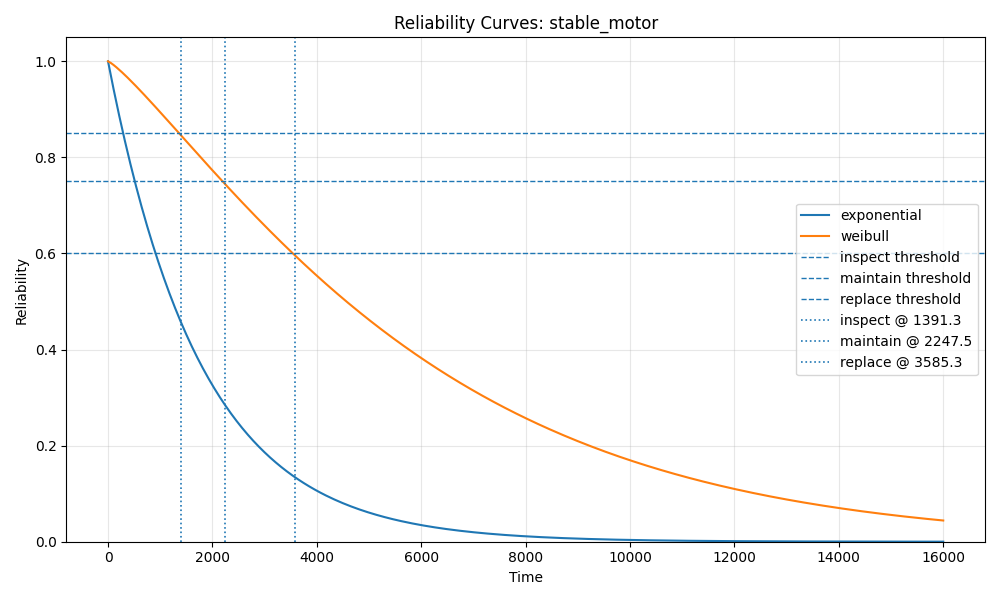
\includegraphics[width=\textwidth]{../results/evals/stable_motor_both/stable_motor_reliability.png}
\caption{stable\_motor}
\end{subfigure}
\hfill
\begin{subfigure}[t]{0.48\textwidth}
\centering
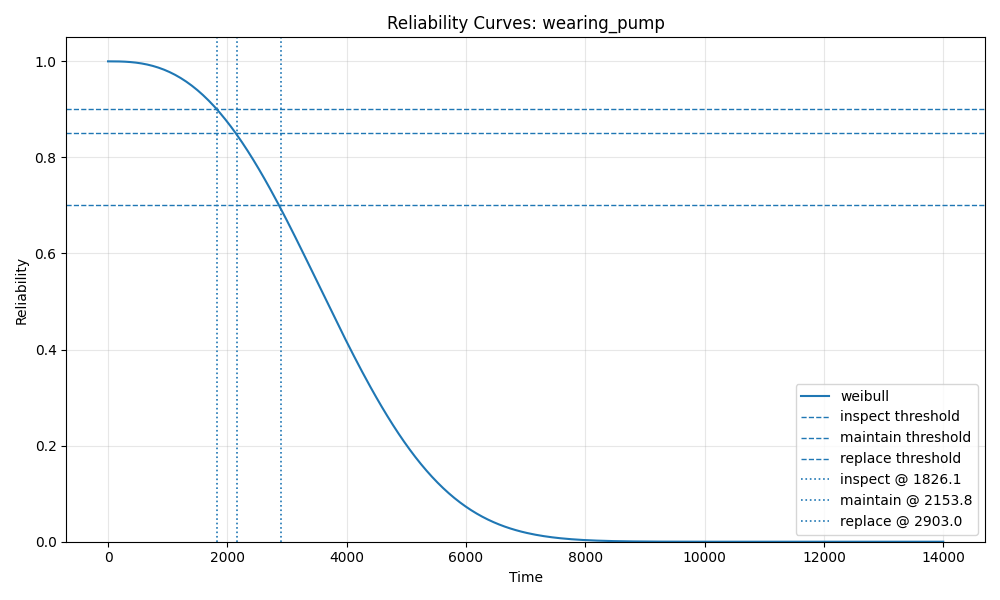
\includegraphics[width=\textwidth]{../results/evals/wearing_pump_weibull/wearing_pump_reliability.png}
\caption{wearing\_pump}
\end{subfigure}

\vspace{0.5cm}

\begin{subfigure}[t]{0.48\textwidth}
\centering
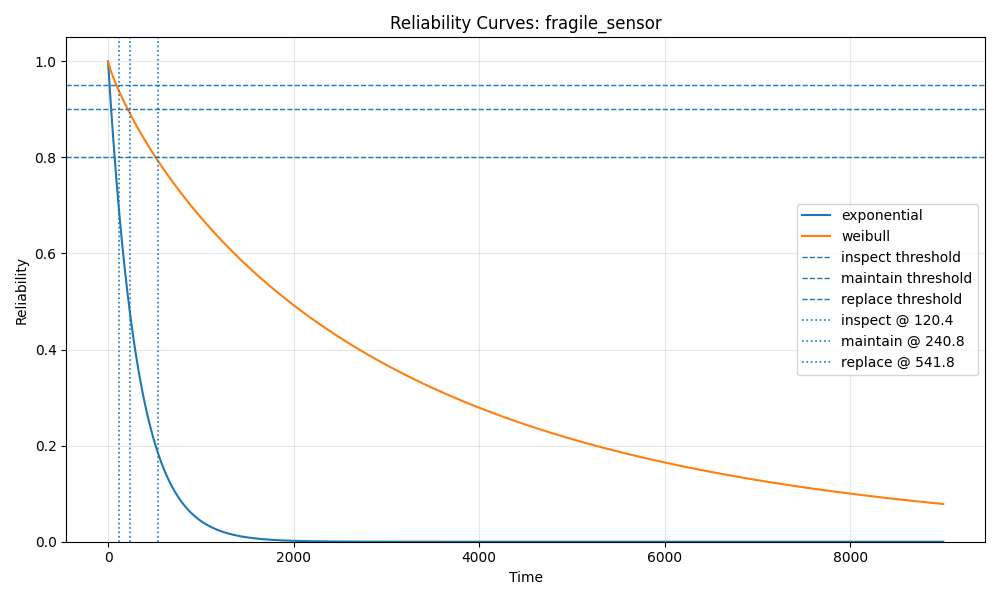
\includegraphics[width=\textwidth]{../results/evals/fragile_sensor_both/fragile_sensor_reliability.png}
\caption{fragile\_sensor}
\end{subfigure}
\hfill
\begin{subfigure}[t]{0.48\textwidth}
\centering
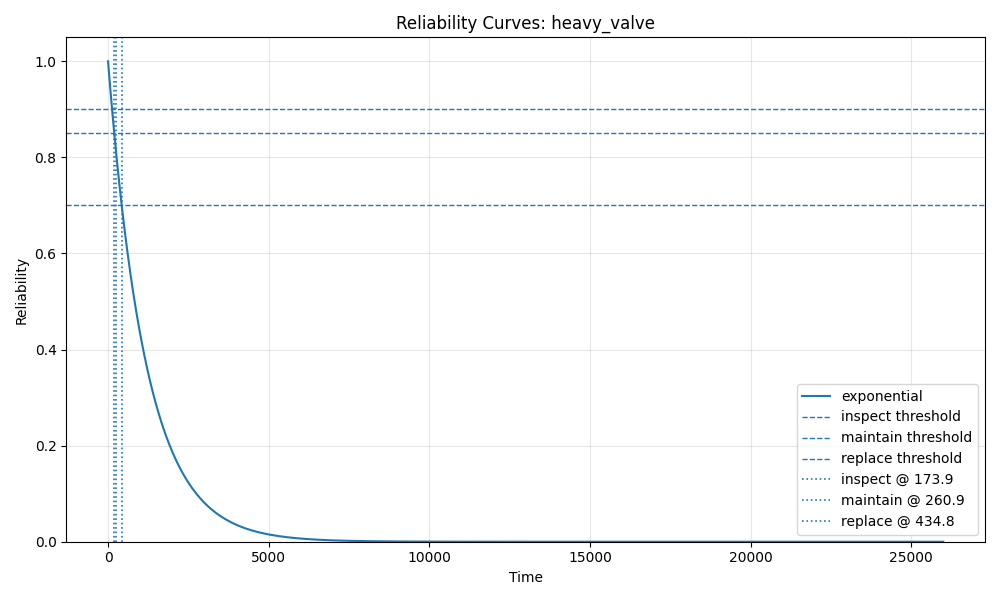
\includegraphics[width=\textwidth]{../results/evals/heavy_valve_exponential/heavy_valve_reliability.png}
\caption{heavy\_valve}
\end{subfigure}
\caption{Representative single-component reliability studies, Part I}
\label{fig:single_one}
\end{figure}

\begin{figure}[H]
\centering
\begin{subfigure}[t]{0.48\textwidth}
\centering
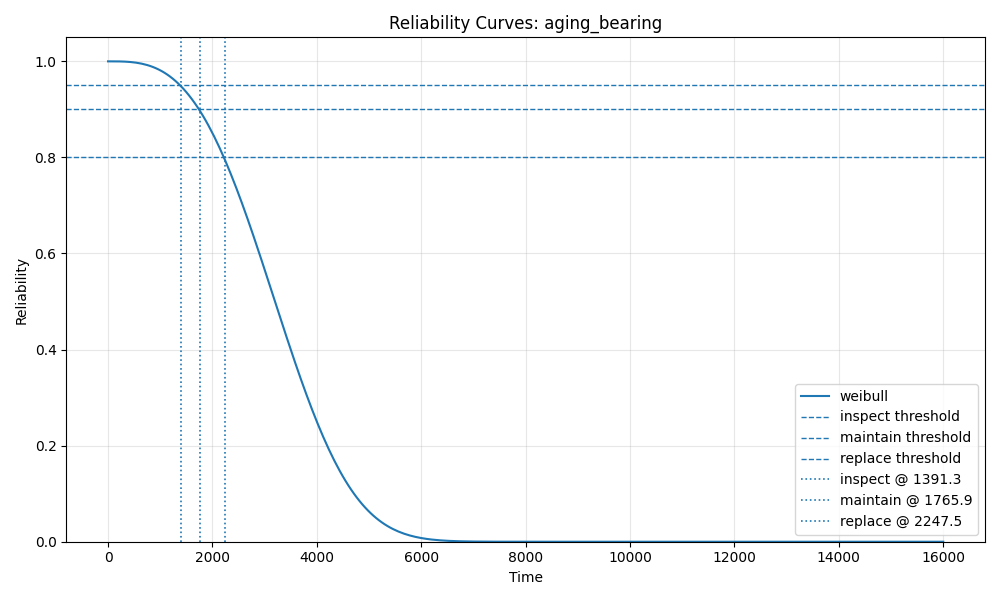
\includegraphics[width=\textwidth]{../results/evals/aging_bearing_weibull/aging_bearing_reliability.png}
\caption{aging\_bearing}
\end{subfigure}
\hfill
\begin{subfigure}[t]{0.48\textwidth}
\centering
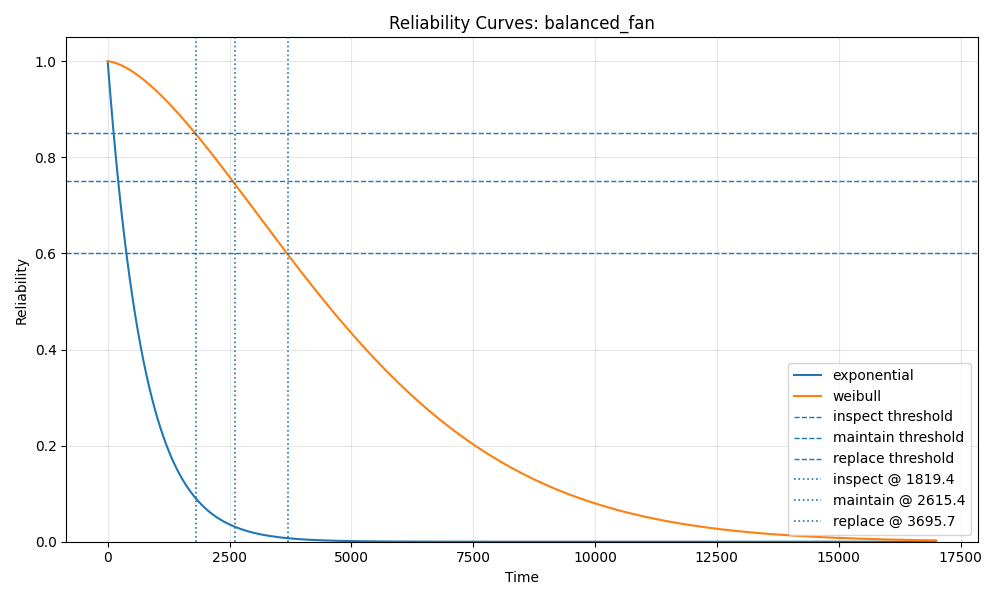
\includegraphics[width=\textwidth]{../results/evals/balanced_fan_both/balanced_fan_reliability.png}
\caption{balanced\_fan}
\end{subfigure}
\caption{Representative single-component reliability studies, Part II}
\label{fig:single_two}
\end{figure}

\section{Comparison Mode Results}
Comparison mode was used to rank six components under three model assumptions. The most important result is the gap between the Weibull and exponential runs. Under Weibull modeling, the slowest-to-fail assets retain acceptable reliability for much longer. Under exponential modeling, the inspect times compress sharply because every asset is treated as if its failure hazard is constant from the start.

\begin{table}[H]
\centering
\caption{Inspect-time sensitivity to model choice in comparison mode}
\label{tab:model_sensitivity}
\begin{tabular}{lrr}
\toprule
Component & Weibull Inspect Time & Exponential Inspect Time \\
\midrule
stable\_motor & 1484.95 & 441.47 \\
wearing\_pump & 1806.02 & 160.54 \\
fragile\_sensor & 120.40 & 80.27 \\
heavy\_valve & 1966.56 & 280.94 \\
aging\_bearing & 1364.55 & 80.27 \\
balanced\_fan & 1765.89 & 361.20 \\
\bottomrule
\end{tabular}
\end{table}

Two operational interpretations follow from Table~\ref{tab:model_sensitivity}:

\begin{enumerate}
\item \texttt{fragile\_sensor} remains the highest-risk asset regardless of model choice. Its inspect window is extremely short in both cases.
\item \texttt{heavy\_valve}, \texttt{stable\_motor}, and \texttt{balanced\_fan} are highly model-sensitive. A conservative exponential assumption shortens the action window by a factor of roughly four to seven.
\end{enumerate}

\begin{figure}[H]
\centering
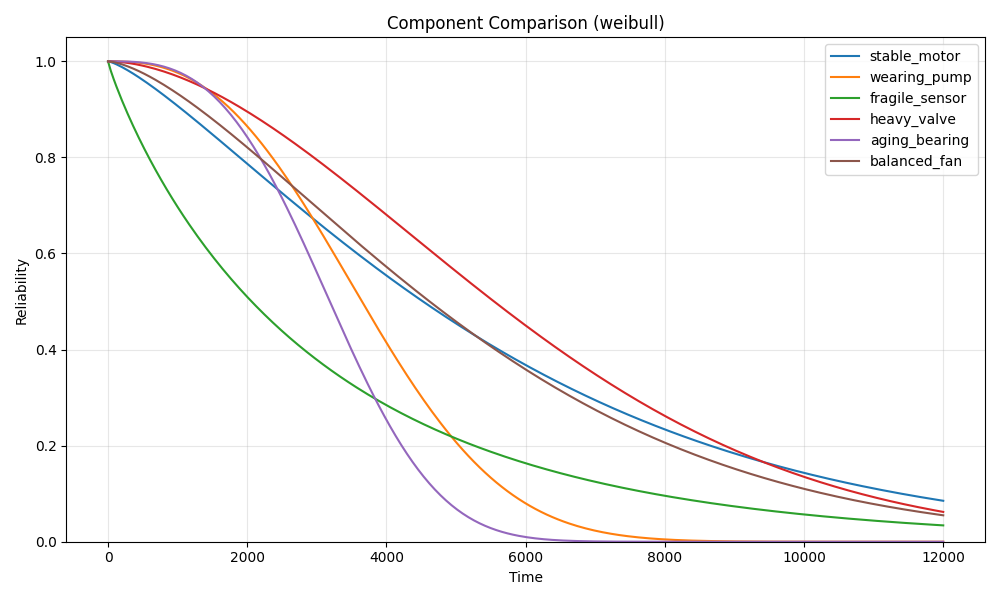
\includegraphics[width=0.8\textwidth]{../results/evals/compare_weibull/comparison_overlay.png}
\caption{Comparison overlay using Weibull reliability}
\label{fig:compare_weibull}
\end{figure}

\begin{figure}[H]
\centering
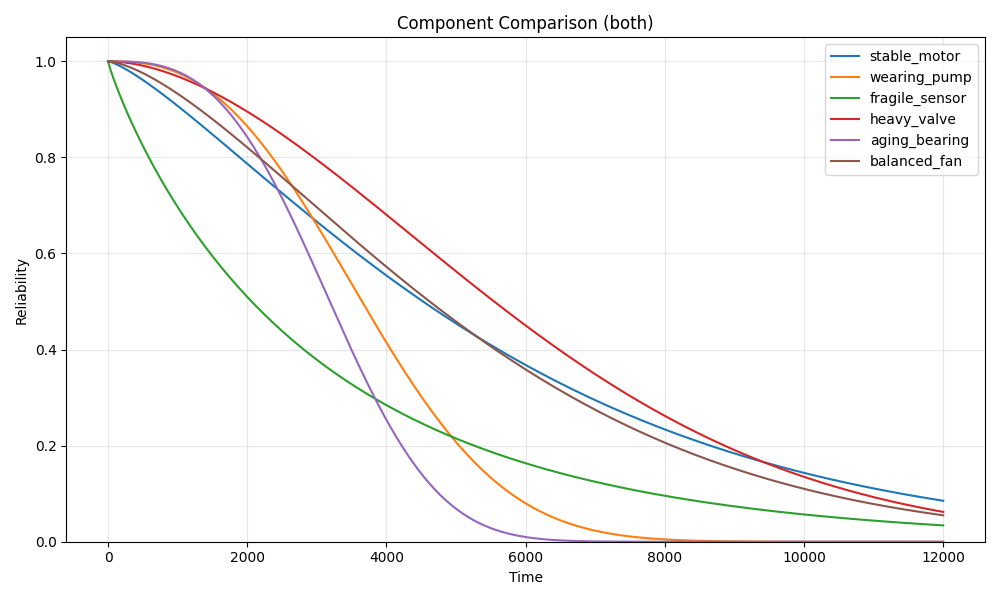
\includegraphics[width=0.8\textwidth]{../results/evals/compare_both/comparison_overlay.png}
\caption{Comparison overlay using combined exponential and Weibull runs for per-component figures}
\label{fig:compare_both}
\end{figure}

\begin{figure}[H]
\centering
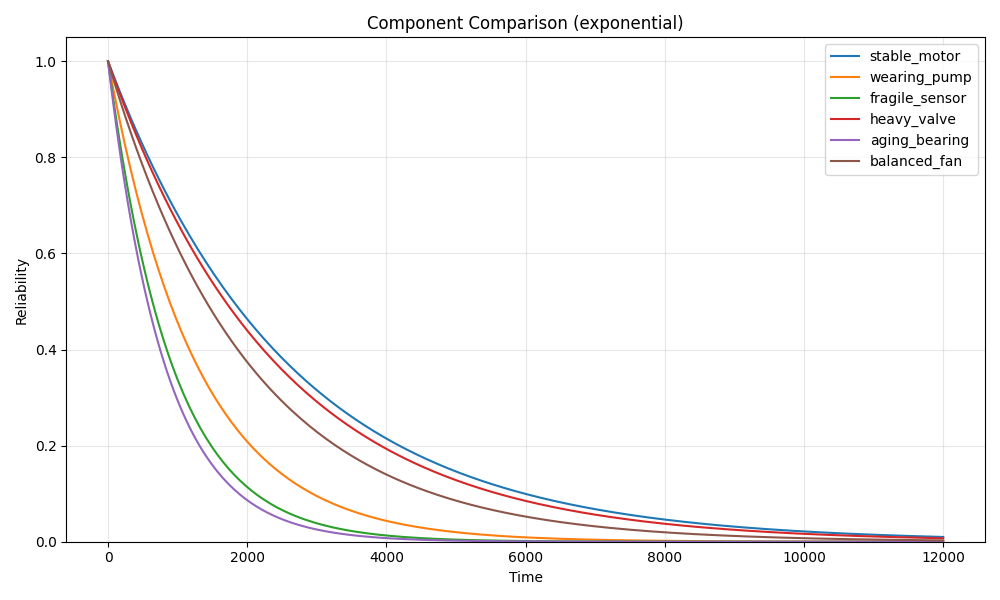
\includegraphics[width=0.8\textwidth]{../results/evals/compare_exponential/comparison_overlay.png}
\caption{Comparison overlay using exponential reliability}
\label{fig:compare_exponential}
\end{figure}

\section{Discussion}
The evaluation supports three conclusions.

\begin{enumerate}
\item The CLI works end to end. Every run produced the expected metrics table, recommendation table, JSON summary, and PNG figure in its designated output folder.
\item The tool is sensitive to both data profile and threshold policy. High-criticality assets and high observed failure counts lead to immediate recommendations, while low-criticality and low-hazard assets preserve longer maintenance windows.
\item Model selection matters in practice. Exponential modeling is consistently more aggressive in these experiments because it applies a constant hazard immediately, whereas Weibull modeling can defer action for components whose fitted shape parameter implies slower early degradation.
\end{enumerate}

\section{Limitations}
These datasets are synthetic, so the evaluation demonstrates software behavior rather than domain-validated maintenance policy. The runs also used user-supplied Weibull parameters instead of estimating them from raw time-to-failure samples. For production deployment, the next step would be to fit parameters from historical maintenance logs and compare the recommendations against actual failure outcomes.

\section{Conclusion}
The repository now contains a functioning maintenance optimization CLI, reproducible datasets, saved evaluation outputs, and a paper-style LaTeX report. The results are internally consistent and show that the tool can move from CSV input to maintenance recommendations and plots without manual intervention.

\end{document}
